\subsubsection{07.01.15}

\begin{enumerate}
	\item Время начала и окончания собрания: 15:00 - 20:00
	
	\item Цели собрания: 
	\begin{enumerate}
		\item Установить на механизм опрокидывания ковша один мощный сервопривод.
		
		\item Заменить неисправный привод (задний правый).
		
		\item Установить на МЗК откосы для центровки подвижной корзины.
	\end{enumerate}
	
	\item Проделанная работа:
	\begin{enumerate}
		
	  \item Одной из задач, сформулированных после последних соревнований, было возврапщение к концепции ковша, разработанной 1 декабря 2014 года. Тогда у нас не было возможности ее реализовать, но сейчас мы располагаем всем необходимым для претворения ее в жизнь.
	  \begin{figure}[H]
	  	\begin{minipage}[h]{1\linewidth}
	  		\center{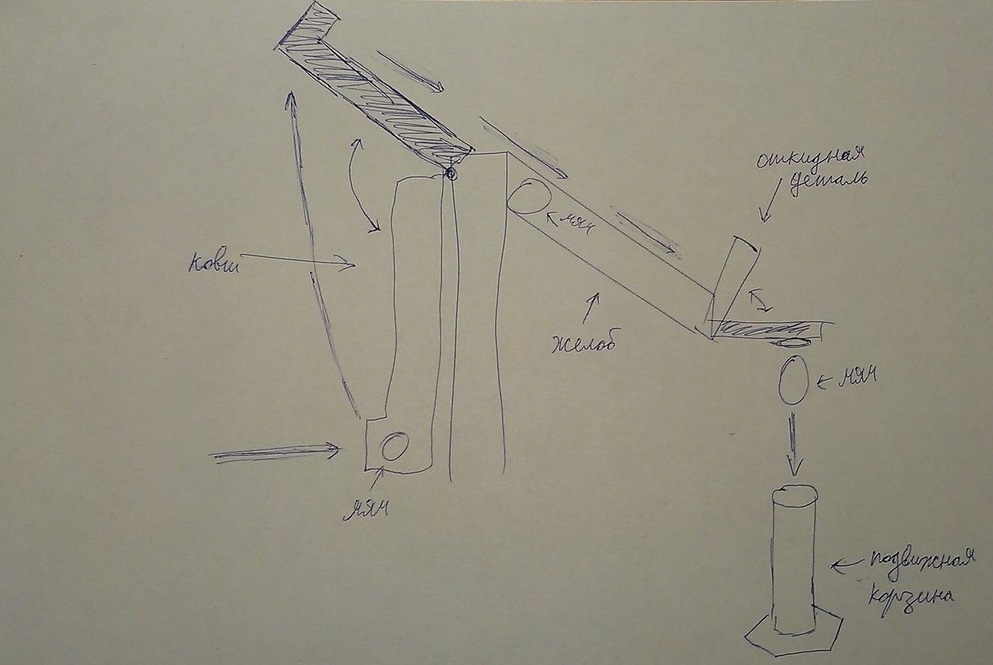
\includegraphics[scale=0.2]{days/07.01.15/images/01}}
	  		\caption{Новый сервопривод}
	  	\end{minipage}
	  \end{figure}
	  
	  \item Для того, чтобы было возможно перенести механизм опрокидывания ковша на верхнюю часть мебельной рейки, необходимо было приобрести более мощный сервопривод, способный опрокинуть ковш в таком положении. Мы остановили свой выбор на модели, по размерам идентичной стандартному сервоприводу, но имеющей усилие в 17 кг/см против стандартных 4 кг/см. Данный сервопривод был нами приобретен к сегодняшнему занятию, однако установить его сегодня не удалось из-за того, что времени на это не хватило.
	  \begin{figure}[H]
	  	\begin{minipage}[h]{1\linewidth}
	  		\center{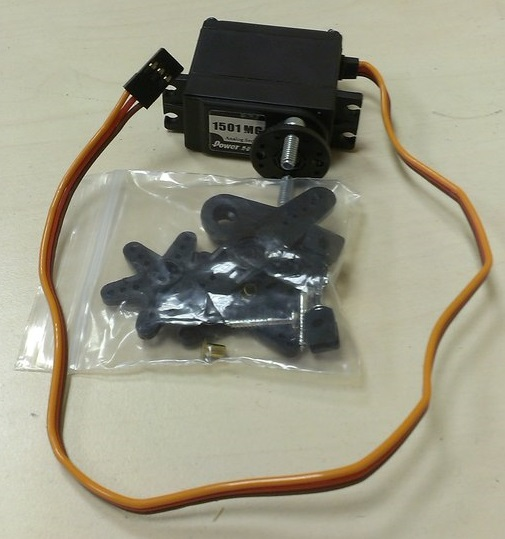
\includegraphics[scale=0.2]{days/07.01.15/images/02}}
	  		\caption{Новый сервопривод}
	  	\end{minipage}
	  \end{figure}
	  	
	  \item Сломанный привод заменен.
	  
	  \item Новый привод протестирован. Результат положительный: привод работает, как надо.
	  
	  \item Были установлены откосы для центровки корзин из обрезков пластиковой бутылки.
      \begin{figure}[H]
      	\begin{minipage}[h]{1\linewidth}
      		\center{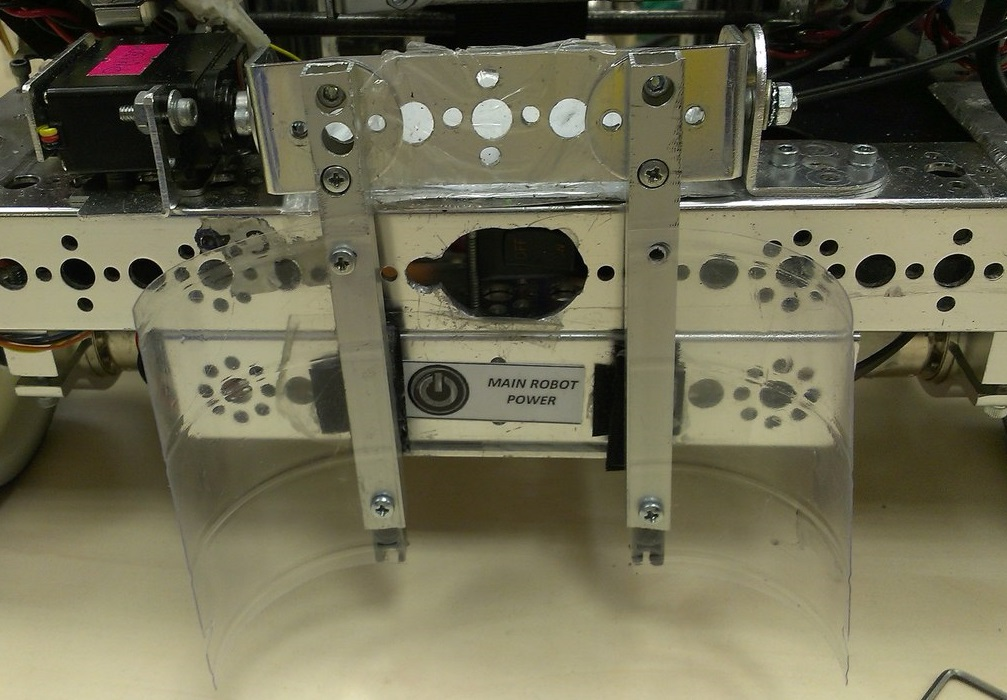
\includegraphics[scale=0.2]{days/07.01.15/images/03}}
      		\caption{Откосы для центровки корзины}
      	\end{minipage}
      \end{figure}	
      
 	\end{enumerate}
 	\item Итоги собрания:
 	\begin{enumerate}
 		
 		\item Сервопривод не установлен.
 		
 		\item Неисправный мотор заменен.
 		
 		\item Откосы для центровки корзины установлены.
 		 
 	\end{enumerate}
 	\item Задачи для последующих собраний:
 	\begin{enumerate}
 		
 		\item Заменить сломанную направляющую.
 		
 		\item Установить на механизм опрокидывания ковша мощный сервопривод.
 		
 		\item Установить ковш на новый сервопривод и испытать механизм опрокидывания в действии.
 				
 	\end{enumerate}
\end{enumerate}
\fillpage